\chapter{Fast Training Algorithms for SVM+}
\label{ch:svmplus}
%\documentclass[10pt,twocolumn,letterpaper]{article}


The advance speed of a field such as computer vision is partly determined by how fast researchers can evaluate new ideas on new tasks and new data. One of the main obstacles on the way is the time-consuming training process, especially given the fact that a large portion of vision problems are highly complex.  Thus, fast training algorithms for standard vision approaches are of a strong need.  In this chapter, we examine this problem for Learning Using Privileged Information~\citep{SVMplus_vapnik}, and propose fast training algorithms for the standard algorithm SVM+~\citep{SVMplus_vapnik}, making its training more affordable.  

\section{Introduction}  
Many computer vision tasks contain privileged information that only
exists in the training data, and not available during the test
stage. For example, the training images of many datasets for image
recognition are annotated with priviledged information such as
\emph{attributes}, \emph{object bounding boxes}, \emph{textual
  descriptions}, \emph{depth information}.  Although the raw test
images in the real-world applications are not associated with such
information, it has been demonstrated that such information is
useful for learning classifiers with better recognition
performance~\citep{Feyereisl2015,Lampert2013,RankTransfer,SVMplus_vapnik,Wang2015,HuaGang2014}.

This problem is known as the \emph{Learning Using Privileged
  Information (LUPI)} problem~\citep{SVMplus_vapnik}. Different from
the traditional learning paradigm, where the training data and the
test data have the same representation, LUPI leverages training data
containing additional information that is only available during the
training process, not in the testing process. Such additional
information in the training data is referred to as privileged
information or hidden information.

Following the LUPI paradigm, Vapnik and Vashist~\citep{SVMplus_vapnik}
proposed an SVM-like algorithm called \emph{SVM+}, in which they
replace the slack variables in the standard SVM with a slack function
defined in the privileged feature space. Through the slack function,
the additional privileged information is used to model the loss
function, which guides the hyperplane learning in the main feature
space. In contrast, the slack variables in the standard SVM are only
constrained to non-negative values, which is often less effective than
the slack function in SVM+.

% Such guidance is useful because
% the privileged information often explains the learning tasks from a
% different perspective.


Although SVM+ can be formulated as a quadratic programming problem in
the dual form similarly as the standard SVM, it is still non-trivial
to efficiently solve it, because the introduction of the slack
function leads to more constraints, and makes the number of dual
variables doubled. While an SMO-style algorithm was developed in
\citep{Pechyony2010}, the working set selection method is complicated,
and the algorithm is also slow in practice. Moreover, it is unclear
how to apply it to linear SVM+ without calculating the kernel matrix,
which is becoming more crucial, due to rapidly increasing data in
real-world applications.

In this work, we propose two efficient algorithms for solving linear
SVM+ and kernel SVM+, respectively. In particular, inspired by linear
SVM \citep{DCD_linearsvm}, we augment the feature vector with an
additional constant element, and absorb the bias term in the decision
function into the weight vector, which leads to a dual form with
simpler constraints. The new linear SVM+ formulation can be
efficiently solved by using the dual coordinate descent method, in a
similar way to linear SVM. For kernel SVM+, we further propose to
apply the $\ell_2$-loss, which leads to a simpler optimization problem
in the dual form with only half of dual variables when compared with
the original SVM+. More interestingly, we show that the resultant dual
form is in analogy to one-class SVM, which can thus be efficiently
solved using the efficient sequential minimal optimization (SMO)
algorithm~\citep{Platt98sequentialminimal} with the existing
state-of-the-art SVM solvers such as
LIBSVM~\citep{svm_workingset,libsvm}.

We implement our algorithms for linear and kernel SVM+ based on
LIBLINEAR~\citep{liblinear} and LIBSVM~\citep{libsvm}, respectively. We
conduct extensive experiments on three tasks: digit recognition on the
MNIST+ dataset~\citep{SVMplus_vapnik}, scene recognition on the
Scene-15 dataset~\citep{scene-15}, and web image retrieval on the
NUS-WIDE dataset~\citep{NUSWIDE}. The results demonstrate that our
proposed algorithms achieve significant speed-up than the
state-of-the-art solvers for solving the linear and kernel SVM+
problems.

% The main contribution of this work is two efficient algorithms for solving the linear and kernel SVM+ problems. The software will be released after the paper is published. We believe that our work will be helpful for exploring the effectiveness of LUPI in more real-world computer vision tasks in the future.

\section{Related Work}
Learning Using Privileged Information (LUPI), as a new
learning paradigm, was first proposed by Vapnik and
Vashist~\citep{SVMplus_vapnik}, therein with the SVM+ algorithm. After
that, many variants of SVM+ have been proposed for solving different
tasks~\citep{MTLSVMPLUS,MetricPI,itmlplus,RankTransfer,Wang2015,Li2014ECCV}. In~\citep{MTLSVMPLUS},
Liang and Cherkassky developed a multi-task learning approach based on
SVM+. In \citep{MTMCSVMPLUS}, a multi-task multi-class extension of
SVM+ was proposed. Fouad~\etal~\citep{MetricPI} designed a two-step
approach for metric learning, and Xu~\etal~\citep{itmlplus} formulated
a convex formulation for metric learning using privileged information
based on the information theory metric learning (ITML)
method. Sharmanska~\etal~\citep{RankTransfer} proposed the Rank
Transfer method for utilizing privileged information, and demonstrated
the effectiveness of privileged information in various computer vision
tasks. In \citep{Li2014ECCV}, Li~\etal extended SVM+ to the
multi-instance learning scenario for image retrieval and object
recognition by learning using web data. In~\citep{Wang2015}, Wang~\etal
proposed a classifier learning algorithm for utilizing privileged
information. In \citep{Feyereisl2015}, Feyereisl~\etal extended
structure SVM to exploiting privileged information for object
localization.

Vapnik and Vashist also showed that SVM+ has a faster convergence rate
than the standard SVM method under certain
conditions~\citep{SVMplus_vapnik}. A more thorough theoretic study of
SVM+ can be found in \citep{LUPIThoery}. In~\citep{Vapnik2015}, two
mechanisms for LUPI are further
explained. Lapin~\etal~\citep{lapin2014learning} also discovered the
relationship between SVM+ and weighted SVM, while
Li~\etal~\citep{Li2014ECCV} discussed the connection of the
unsupervised domain adaptation method and SVM+.

One closely related work is \citep{Pechyony2010}, in which an SMO-style
algorithm was developed for the SVM+ problem. However, as the two sets
of dual variables introduced for the constraints related to the main
and privileged features in the primal form are tangled together in the
constraints of dual problem, it is non-trivial to design the working
set selection method for the SMO algorithm, and leads to a complicated
algorithm that is less efficient in practice. Moreover, it is also
unclear that how to apply the the SMO-style algorithm for solving the
linear SVM+ problem without calculating the kernel matrix. In
contrast, in this work, by absorbing the bias term into the weight
vector of the SVM+ classifier, we arrive at an optimization problem
with simpler constraints in the dual form. Thus, the conventional dual
coordinate descent algorithm can be applied to efficiently solve
linear SVM+. Moreover, for the SVM+ form, we further apply the
$\ell_2$-loss and obtain a smaller dual problem with only a half of
dual variables of the original SVM+ formulation. The new dual form
shares a similar formulation with one-class SVM, and thus can be
solved by using the SMO algorithm implemented in the existing SVM
solvers such as LIBSVM~\citep{libsvm} without developing any new
specific SMO algorithm. We demonstrate that our proposed two
algorithms are more efficient than the SMO-style algorithm in
\citep{Pechyony2010}.

In a more broader context, there are  works proposed for solving
tasks in which training and test data use asymmetric information source,
which are less related to
SVM+~\citep{Chen2013,ChenLin2014CVPR, metric:imitation,Ding2014,SuTransfer,DistillingCNN,lsda,Lampert2013,Srivastava2012,HuaGang2014}.


\section{Learning Using Privileged Information}
In the following, we denote a vector (\resp, matrix)
with a lower (\resp, upper) case letter in boldface. For example, $\a$
represents a vector, and $\A$ a matrix. The transpose of a vector or
matrix is denoted by using the superscript $'$. We use $\0_n, \1_n \in
\bbR^n$ to represent the column vector with $n$ zeros and ones,
respectively. We also simply use $\0$ and $\1$ instead of $\0_n$ and
$\1_n$, when the dimensionality is obvious. Moreover, $\a\circ \b$ (\resp,
$\A \circ \B$) denotes the element-wise product between two vectors
(\resp, matrices).

In the Learning Using Privileged Information (LUPI)
paradigm~\citep{SVMplus_vapnik}, the training samples contain
additional information that is not available in the test
stage. Formally, we represent the training data as $\{(\x_i,
\tilde{\x}_i, y_i)|i = 1, \ldots, n\}$, where $n$ is the total number
of training samples, $\x_i \in \bbR^D$ is the main feature vector of
the $i$-th training sample with $D$ being the feature dimensionality,
$\tilde{\x} \in \bbR^{\tilde{D}}$ is the corresponding privileged
feature vector with $\tilde{D}$ being its dimension. The goal of LUPI
is to learn a decision function $f(\x)$ for classifying any test
sample $\x \in \bbR^D$ in the main feature space.

In \citep{SVMplus_vapnik}, an SVM based approach called \emph{SVM+} was proposed. Similar to SVM, the decision function in SVM+ is represented as $f(\x) = \w'\phi(\x) + b$, where $\phi(\cdot)$ is a feature mapping induced by the kernel on training data, $\w$ is the weight vector, and $b$ is the bias term. The objective of SVM+ can be written as,
\begin{eqnarray}
\min_{\tilde{\w}, \tilde{b}, \w, b}\!\!\!\!&&\!\!\!\!\frac{1}{2}\left(\|\w\|^2 + \gamma\|\tilde{\w}\|^2\right)+ C\sum_{i=1}^{n}\xi(\tilde{\w}, \tilde{b}, \psi(\tilde{\x}_i))\quad\label{eqn:PL}\\
\mbox{s.t.}\!\!\!\!&&\!\!\!\!y_i(\w'\phi(\x_i) + b) \geq 1 - \xi(\tilde{\w}, \tilde{b}, \psi(\tilde{\x}_i)),\label{eqn:PL_cons1}\\
\!\!\!\!&&\!\!\!\!\xi(\tilde{\w}, \tilde{b}, \psi(\tilde{\x}_i)) \geq 0,\label{eqn:PL_cons2}
\end{eqnarray}
where $\xi(\tilde{\w}, \tilde{b}, \psi(\tilde{\x}_i)) = \tilde{\w}'\psi(\tilde{\x})+\tilde{b}$ is the slack function defined in the privileged feature space, $\psi(\cdot)$ is the feature mapping function for the privileged features, and $\tilde{\w}$ and $\tilde{b}$ are respectively the weight vector and bias term for the slack function. It can be observed that SVM+ replaces the slack variables in the standard SVM formulation with the slack function $\xi(\tilde{\w}, \tilde{b}, \psi(\tilde{\x}_i))$. As a result, the loss occurred by the training samples $\x_i$ can be regularized by the privileged information $\tx_i$, therefore the hyperplane of SVM+ classifier can be tuned by using the privileged information during the training process.

Let us introduce two sets of dual valuables $\{\alpha_i|_{i=1}^n\}$ and  $\{\zeta_i|_{i=1}^n\}$ for the constraints in Equation~\ref{eqn:PL_cons1} and Equation~\ref{eqn:PL_cons2}, respectively, and also denote two vectors $\ba = [\alpha_1, \ldots, \alpha_n]'\in \bbR^n$ and $\bz = [\zeta_1, \ldots, \zeta_n]'\in \bbR^n$.  We arrive at the dual form of SVM+,
\begin{eqnarray}\label{eqn:PL_dual}
\min_{(\bz, \ba) \in \cA} && \frac{1}{2}(\ba\circ\y)'\K(\ba\circ\y) -\1'\ba  \\
&& + \frac{1}{2\gamma}(\ba + \bz - C\1)'\tilde{\K}(\ba + \bz - C\1) \nonumber,
\end{eqnarray}
where $\cA = \{(\bz, \ba)| \y'\ba = 0, \1'(\ba+\bz-C\1) = 0, \ba \geq 0, \bz \geq 0\}$ is the feasible set of $(\ba, \bz)$, $\K\in \bbR^{n\times n}$ is the kernel matrix based on the  main training features with each element being $K_{ij} = \phi(\x_i)'\phi(\x_j)$, and $\tK\in \bbR^{n\times n}$ is the kernel matrix based on the privileged features with each element being $\tilde{K}_{ij} = \psi(\tx_i)'\psi(\tx_j)$. After solving the above problem, the weight vectors $\w$ and $\tw$ can be reconstructed based on the Karush-–Kuhn-–Tucker (KKT) conditions as,
\begin{eqnarray}
\w &=& \sum_{i=1}^n \alpha_iy_i\phi(\x_i) \label{eqn:equation_w},\\
\tw &=& \frac{1}{\gamma}\sum_{i=1}^n (\alpha_i+\zeta_i - C)\psi(\tx_i) \label{eqn:equation_tw}.
\end{eqnarray}

Although the dual problem in Equation~\ref{eqn:PL_dual} is a quadratic programming problem, solving it with the existing optimization toolboxes is certainly undesirable for real-world visual recognition tasks. However, it is non-trivial to develop efficient algorithm like the SMO algorithm for solving the standard SVM. The main difficulty comes from the constraint $\1'(\ba+\bz-C\1) = 0$, in which two sets of dual variables are tangled together, which makes the working set selection method become complicated~\citep{Pechyony2010}.

\section{Dual Coordinate Descent Algorithm for Solving Linear SVM+}\label{sec:linear_svmplus}
In this section, we present the dual coordinate descent method for solving the linear SVM+. In particular, we absorb the bias term into the weight vector $\w$ by appending a constant entry of $1$ to each feature vector, \ie, $\x\leftarrow [\x', 1]'$, and $\w\leftarrow[\w', b]'$ for the main features, and $\tx\leftarrow [\tx', 1]'$, and $\tw\leftarrow[\tw', \tilde{b}]'$ for privileged information. For ease of presentation, we still use $\w$ and $\x$ (\resp, $\tw$, $\tx$) to represent the weight vector and feature vector for the main (\resp, privileged) features.

Now, the objective of linear SVM+ can be reformulated as follows,
\begin{eqnarray}\label{eqn:linear_svmplus}
\min_{\tilde{\w}, \w} && \frac{1}{2}\left(\|\w\|^2 + \gamma\|\tilde{\w}\|^2\right)+ C\sum_{i=1}^{n}\tw'\tx\\
\mbox{s.t.} && y_i\w'\x_i \geq 1 - \tw'\tx,\nonumber\\
&& \tw'\tx_i \geq 0,\nonumber
\end{eqnarray}
and its dual form can be written as,
\begin{eqnarray}\label{eqn:linear_svmplus_dual}
\min_{(\bz, \ba) \in \cA} && \frac{1}{2}(\ba\circ\y)'\K(\ba\circ\y) -\1'\ba  \\
&&  + \frac{1}{2\gamma}(\ba + \bz - C\1)'\tilde{\K}(\ba + \bz - C\1),\nonumber
\end{eqnarray}
where the feasible set becomes $\cA = \{(\bz, \ba)| \ba \geq 0, \bz \geq 0\}$, $\K \in \bbR^{n\times n}$ is the linear kernel matrix of main features defined as $K_{ij} = \x_i'\x_j$, and $\tK\in \bbR^{n\times n}$ is the linear kernel matrix of privileged features defined as $\tilde{K}_{ij} = \tx_i'\tx_j'$. Compared to the dual form of the original SVM+ formulation~Equation~\ref{eqn:PL_dual}, the objective function remains the same, but we do not have the constraints $\y'\ba = 0, \1'(\ba+\bz-C\1) = 0$ in Equation~\ref{eqn:linear_svmplus_dual}, after absorbing of the bias terms in Equation~\ref{eqn:linear_svmplus}. The weight vectors $\w$ and $\tw$ can be represented using the dual variables in the same way as in Equation~\ref{eqn:equation_w} and Equation~\ref{eqn:equation_tw} without using the feature mapping functions (\ie, we can set $\phi(\x_i) = \x_i$ and $\psi(\tx_i) = \tx_i$.

Let us define $\Q = \begin{bmatrix}\K\circ(\y\y') + \frac{1}{\gamma}\tK & \frac{1}{\gamma}\tK\\ \frac{1}{\gamma}\tK & \frac{1}{\gamma}\tK\end{bmatrix} \in \bbR^{2n\times 2n}$, $\bb = [\ba', \bz']' \in \bbR^{2n}$, $\e = [(\1+\frac{C}{\gamma}\tK\1)', (\frac{C}{\gamma}\tK\1)']' \in \bbR^{2n}$, the problem in Equation~\ref{eqn:linear_svmplus_dual} can be rewritten in a more concise form as,
\begin{eqnarray}
\min_{\bb} && \frac{1}{2}\bb'\Q\bb -\e'\bb\label{eqn:linear_svmplus_dual2}\\
\mbox{s.t.}&& \bb \geq 0.\nonumber
\end{eqnarray}

Now we develop a coordinate descent algorithm for the problem in Equation~\ref{eqn:linear_svmplus_dual2} similarly as that for linear SVM~\citep{DCD_linearsvm}. In the dual coordinate descent algorithm, we iteratively update one entry of $\bb$ each time. This process is repeated until the stopping criterion is reached.

In particular, let us denote $f(\bb) = \frac{1}{2}\bb'\Q\bb -\e'\bb$, and we propose to update the $i$-th entry as $\beta_i\leftarrow \beta_i + d$, where $d$ is a scalar variable that needs to be solved. By defining $\bd^{(i)} = [0, \ldots, 0, 1, 0, \ldots, 0]$ as the vector with all zeros except the $i$-th entry being one, the subproblem for solving $d$ can be formulated as
\begin{eqnarray}
\min_{d} f(\bb + d\bd^{(i)}) \quad \mbox{s.t.}\,\,\bb +  d\bd^{(i)} \geq 0,\label{eqn:linear_svmplus_sub}
\end{eqnarray}
which has an analytic solution as follows,
\begin{eqnarray}
d = \max(- \beta_i, - \frac{\nabla_i f(\bb)}{Q_{ii}}) \label{eqn:linear_svmplus_calc_d}
\end{eqnarray}
where $Q_{ii}$ is the $(i, i)$-th entry of the matrix $\Q$ in Equation~\ref{eqn:linear_svmplus_dual2}, and $\nabla_if(\bb)$ is the gradient of $f(\bb)$ \wrt $\beta_i$.

Now we discuss how to efficiently calculate the right-hand side of Equation~\ref{eqn:linear_svmplus_calc_d}. The scalar $Q_{ii}$ can be pre-computed efficiently, so the major problem is the calculation of $\nabla_i f(\bb)$. In particular, the gradient of $f(\bb)$ can be written as $\nabla f(\bb) = \Q\bb - \e$. Then, for any given index $i$, the gradient of $f(\bb)$ \wrt $\beta_i$ can be calculate as,
\begin{eqnarray}\label{eqn:linear_svmplus_grad}
\nabla_if(\bb) = (\Q\bb)_i - e_i = \sum_{j=1}^{2n}Q_{ij}\beta_j - e_i,
\end{eqnarray}
where $Q_{ij}$ is the $(i, j)$-th element of the matrix $\Q$, and $e_i$ is the $i$-th element of the vector $\e$.

We discuss the detailed calculations in two cases. Let us denote a matrix $\H = \K\circ\y\y' \in \bbR^{n\times n}$. For $\forall i = 1,\ldots, n$, we have
\begin{eqnarray}
\sum_{j=1}^{2n}Q_{ij}\beta_j = \sum_{j=1}^nH_{ij}\alpha_j + \frac{1}{\gamma}\sum_{j=1}^n\tilde{K}_{ij}\alpha_j + \frac{1}{\gamma}\sum_{j=1}^n\tilde{K}_{ij}\zeta_j\nonumber
\end{eqnarray}
where $H_{ij}$ is the $(i,j)$-th element of the matrix $\H$. We also have $e_i = 1 +\frac{C}{\gamma}\sum_{j=1}^n\tilde{K}_{ij}$. By applying the KKT conditions \wrt $\w$ and $\tw$ in Equation~\ref{eqn:equation_w} and Equation~\ref{eqn:equation_tw}, the gradient of $f$ \wrt $\beta_i$ in Equation~\ref{eqn:linear_svmplus_grad} can be written as,
\begin{eqnarray}\label{eqn:linear_svmplus_grad_01}
\nabla_if(\bb)_i = y_i\w'\x_i - 1  + \tw'\tx_i, \quad \forall 1\leq i \leq n
\end{eqnarray}
which takes $O(D+\tilde{D})$ time complexity, and it can be further speed-up if the feature vectors $\x$ and $\tx$ are sparse.

%  and $\tw = \frac{1}{\gamma}\sum_{j=1}^n(\alpha_j + \beta_j - C) \tx_j$.
Similarly,  for  $\forall i = n+1, \ldots, 2n$, we have
\begin{eqnarray}
\sum_{j=1}^{2n}Q_{ij}\beta_j &=& \frac{1}{\gamma}\sum_{j=1}^n\tilde{K}_{ij}\alpha_j + \frac{1}{\gamma}\sum_{j=1}^n\tilde{K}_{ij}\zeta_j,\nonumber
\end{eqnarray}
and $e_i = \frac{C}{\gamma}\sum_{j=1}^n\tilde{K}_{ij}$. By using the KKT condition for $\tw$ in Equation~\ref{eqn:equation_tw}, the gradient in Equation~\ref{eqn:linear_svmplus_grad} can be written as,
\begin{eqnarray}\label{eqn:linear_svmplus_grad_02}
\nabla_if(\bb)_i = \tw'\tx_i,\quad \forall n+1\leq i \leq 2n,
\end{eqnarray}
which takes $O(\tilde{D})$ time complexity only, and can also be further speed-up if the feature vector $\tx$ is sparse. This completes the calculation of Equation~\ref{eqn:linear_svmplus_calc_d}.

After solving $d$, we can update the $i$-th dual variable $\beta_i$ by using $\beta_i\leftarrow \beta_i + d$. Considering only one dual variable is modified each time, the weight vectors can be updated efficiently at each iteration. Note that we have $\alpha_i = \beta_i$ when $1\leq i\leq n$, and $\zeta_{i-n} = \beta_{i}$, when $n+1\leq i \leq n$. Based on Equation~\ref{eqn:equation_w} and Equation~\ref{eqn:equation_tw}, the updating rules for $\w$ and $\tw$ can be written as
\begin{eqnarray}
\w  &\leftarrow& \w + dy_i\x_i, \quad \mbox{if\,\,} 1\leq i \leq n\label{enq:update_w}\\
\tw  &\leftarrow& \tw + \frac{1}{\gamma}d\tx_i,\quad \mbox{if\,\,} 1\leq i \leq 2n\label{enq:update_tw}
\end{eqnarray}

We summarize our dual coordinate descent algorithm for solving linear SVM+ in Algorithm~\ref{alg:linear_svmplus}. We first initialize the weight vectors as $\w = \0_{D}$, and $\tw = -\frac{C}{\gamma}\sum_{i=1}^n\tx_i$ (\ie, the solution of $\w$ and $\tw$ when $\ba = \0$ and $\bz = \0$). Then, each time, we randomly pick up an index $i$, and solve $d$ (\ie, the change of $\beta_i$) using Equation~\ref{eqn:linear_svmplus_calc_d}. In particular, when $1 \leq i \leq n$, we calculate the gradient $\nabla_if(\bb)$ using Equation~\ref{eqn:linear_svmplus_grad_01}, and update the weight vectors $\w$ and $\tw$ using Equation~\ref{enq:update_w} and Equation~\ref{enq:update_tw}, respectively; when $n+1 \leq i \leq 2n$, we calculate the gradient $\nabla_if(\bb)$ using Equation~\ref{eqn:linear_svmplus_grad_02} and update the weight vector $\tw$ only using Equation~\ref{enq:update_tw}. The above process is repeated until the objective converges. Actually, the problem in Equation~\ref{eqn:linear_svmplus_dual2} can be treated as a special form of the linear SVM problem discussed in \citep{DCD_linearsvm}, so the convergence of our algorithm follows that of the dual coordinate descent algorithm for linear SVM. We implement our algorithm based on the LIBLINEAR software~\citep{liblinear}.
\begin{algorithm}[t]
   \caption{Dual coordinate descent algorithm for solving the linear SVM+ problem in Equation~\ref{eqn:linear_svmplus}}
   \label{alg:linear_svmplus}
   \begin{algorithmic}[1]
   \REQUIRE  $\{(\x_i, \tx_i, y_i)|_{i=1}^n\}$,  $C$, and $\gamma$.
   \STATE Initialize $\w = \0$, and $\tw = -\frac{C}{\gamma}\sum_{i=1}^n\tx_i$.
   \STATE Set $Q_{ii} = \x_i'\x_i$ for $1 \leq i \leq n$, and $Q_{ii} = \tx_i'\tx_i$ for $n+1\leq i \leq 2n$.
   \REPEAT
      \STATE Randomly pick an index $i$.
      \IF {$1 \leq i \leq n$}
      \STATE  Calculate $\nabla_if(\bb)$ using Equation~\ref{eqn:linear_svmplus_grad_01}.
      \ELSE
      \STATE  Calculate $\nabla_if(\bb)$ using Equation~\ref{eqn:linear_svmplus_grad_02}.
      \ENDIF
      \STATE Calculate $d$ using Equation~\ref{eqn:linear_svmplus_calc_d} based on $Q_{ii}$ and $\nabla_if(\bb)$.
      \IF {$1 \leq i \leq n$}
        \STATE       Update $\w$ using Equation~\ref{enq:update_w}.
      \ENDIF
      \STATE Update $\tw$ using Equation~\ref{enq:update_tw}.
   \UNTIL{The convergence criterion is reached.}
   \ENSURE Weight vectors $\w$ and $\tw$.
\end{algorithmic}
\end{algorithm}

\section{SMO Algorithm for Solving Kernel SVM+}
In this section, we develop an efficient algorithm for solving kernel SVM+ based on the $\rho$-SVM formulation. Similar to linear SVM+, we also augment the feature vector in the nonlinear feature space, so we can absorb the bias term into the weight vector, \ie, $\phi(\x_i) \leftarrow [\phi(\x_i)', 1]'$ and $\w \leftarrow [\w', b]'$ for the main features (\resp,  $\psi(\tx_i) \leftarrow [\psi(\tx_i)', 1]'$ and $\tw \leftarrow [\tw', \tilde{b}]'$ for the privileged features)\footnote{Note we usually do not know the explicit form of $\phi(\cdot)$, but rather the inner product of the augmented features can be simply calculated by adding one, \ie, $\phi(\x_i)'\phi(\x_j)\leftarrow\phi(\x_i)'\phi(\x_j) + 1$, which also means the kernel matrix based on the augmented features can be calculated by $\K \leftarrow \K + \1\1'$. The same approach can be applied to the privileged features. }. For ease of presentation, we still use $\phi(\x_i)$ and $\w$ to denote the nonlinear feature and weight vector for the main features (\resp, $\psi(\tx_i)$ and $\tw$ for privileged features) below.

Specifically, after using the augmented features, the decision function can be represented as $f(\x) = \w'\phi(\x)$.  We use the squared hinge loss for $\rho$-SVM, which leads to the $\ell_2$ loss $\rho$-SVM formulation as follows,
\begin{eqnarray}\label{eqn:l2rhosvm}
\min_{\w, b, \rho} && \frac{1}{2}\|\w\|^2 + \frac{1}{2}C\sum_{i=1}^{n}\xi_i^2 - \rho\\
\mbox{s.t.} && y_i(\w'\phi(\x_i)) \geq \rho - \xi_i.\nonumber
\end{eqnarray}

By replacing each slack variable $\xi_i$ with the slack function $\xi(\tx_i) = \tw'\psi(\tx_i)$, we arrive at the primal form of $\ell_2$-SVM+ as follows,
\begin{eqnarray}\label{eqn:l2rhosvmplus}
\min_{\tilde{\w}, \w, \rho}\!\!\!\!&&\!\!\!\!\frac{1}{2}\left(\|\w\|^2 + \gamma\|\tilde{\w}\|^2\right)+ \frac{1}{2}C\sum_{i=1}^{n}\left(\tilde{\w}'\psi(\tilde{\x}_i)\right)^2 - \rho\nonumber\\
\mbox{s.t.}\!\!\!\!&&\!\!\!\! y_i(\w'\phi(\x_i)) \geq \rho - \tilde{\w}'\psi(\tilde{\x}_i).
\end{eqnarray}

Now we derive the dual form of our $\ell_2$-SVM+ formulation in Equation~\ref{eqn:l2rhosvmplus}. By introducing dual variables $\alpha_1, \ldots, \alpha_n$ for the constraints in Equation~\ref{eqn:l2rhosvmplus}, we write its Lagrangian as follows,
\begin{eqnarray}\label{eqn:l2svmplus_lagrangian}
\cL\!\!\!\!&=&\!\!\!\!\frac{1}{2}\left(\|\w\|^2 + \gamma\|\tilde{\w}\|^2\right)+ \frac{1}{2}C\sum_{i=1}^{n}\left(\tilde{\w}'\psi(\tilde{\x}_i)\right)^2 - \rho\qquad\\
\!\!\!\!&&\!\!\!\!- \sum_{i=1}^n\alpha_i\left(y_i(\w'\phi(\x_i)) - \rho + \tilde{\w}'\psi(\tilde{\x}_i)\right),\nonumber
\end{eqnarray}

Let us denote a vector $\ba = [\alpha_1, \ldots, \alpha_n]'$. By setting the derivatives of Equation~\ref{eqn:l2svmplus_lagrangian} \wrt to the primal variables $\w, \tw, \rho$ to zeros, we obtain the constraint $\ba'\1 = 1$ as well as two KKT conditions for $\w$ and $\tw$ as follows,
\begin{eqnarray}
\w &=& \sum_{i=1}^n\alpha_iy_i\phi(\x_i),\label{eqn:l2rhosvmplus_w}\\
\tilde{\w} &=& \sum_{i=1}^n\alpha_i\left(\gamma\I + C\P\P'\right)^{-1}\psi(\tilde{\x}_i),\label{eqn:l2rhosvmplus_tw}
% C\sum_{i=1}^n\tilde{\phi}(\tilde{\x}_i)\tilde{\phi}(\tilde{\x}_i))'\tilde{\w} - \sum_{i=1}^n\alpha_i\tilde{\phi}(\tilde{\x}_i) = 0,\nonumber
\end{eqnarray}
where $\P = [\psi(\tx_1), \ldots, \psi(\tx_n)]$ is the data matrix of privileged features in the nonlinear feature space.

Substituting the two equations in Equation~\ref{eqn:l2rhosvmplus_w} and Equation~\ref{eqn:l2rhosvmplus_tw} into the Lagrangian in Equation~\ref{eqn:l2svmplus_lagrangian}, we arrive at the dual form of Equation~\ref{eqn:l2rhosvmplus} as follows,
\begin{eqnarray}\label{eqn:l2svmplus_dual}
\min_{\ba} && \frac{1}{2}\ba'(\H + \G)\ba\\
\mbox{s.t.} && \1'\ba = 1, \quad \ba \geq 0,\nonumber
\end{eqnarray}
where $\G = \P'\left(\gamma\I + C\P\P'\right)^{-1}\P$, $\H = \K\circ(\y\y')$, and $\K$ is the kernel matrix of augmented main features with $K_{ij} = \phi(\x_i)'\phi(\x_j)$ being its $(i,j)$-th element. Based on the equation $\left(\gamma\I + C\P\P'\right)^{-1}\P = \P\left(\gamma\I + C\P'\P\right)^{-1}$, we have $ \G = \P'\P\left(\gamma\I + C\P'\P\right)^{-1} = \tK\left(\gamma\I + C\tK\right)^{-1}$, where $\tK$ is the kernel matrix of augmented privileged features with $\tilde{K}_{ij} = \psi(\x_i)'\psi(\x_j)$ being its $(i,j)$-th element. By further applying the Woodbury Identity, we obtain $\G = \frac{1}{C}\I - \frac{1}{C}\left(\I+\frac{C}{\gamma}\tK\right)^{-1}$.

Note the problem in Equation~\ref{eqn:l2svmplus_dual} is a quadratic programming problem with the number of dual variables being $n$, which is only half number of variables in the dual form of the original SVM+ method in Equation~\ref{eqn:PL_dual}. Moreover, the constraints in Equation~\ref{eqn:l2svmplus_dual} are also simpler, so it can be solved by using the efficient SMO algorithm. Actually, the problem in Equation~\ref{eqn:l2svmplus_dual} shares a similar form with one-class SVM in the LIBSVM software~\citep{libsvm}. In particular, we write the dual form of one-class SVM as follows (Eqn. (8) in \citep{libsvm}),
\begin{eqnarray}\label{eqn:oneclass_svm_dual}
\min_{\ba} && \frac{1}{2}\ba'\Q\ba\\
\mbox{s.t.} && \1'\ba = \nu n, \quad 0\leq \ba \leq 1\nonumber,
\end{eqnarray}
where $\Q$ is the kernel matrix in one-class SVM, $\nu$ is a predefined parameter, $n$ is total the number of training samples.  Note the constraints $\ba \geq \0$ and $\1'\ba = 1$ in Equation~\ref{eqn:l2svmplus_dual} imply $0 \leq \ba \leq 1$. By setting $\Q = (\H + \G)$ and $\nu =  \frac{1}{n}$, the dual problem of $\ell_2$-SVM+ in Equation~\ref{eqn:l2svmplus_dual} can be converted to the optimization problem in Equation~\ref{eqn:oneclass_svm_dual}. Therefore, we ignore the details of the SMO algorithm here, and employ the SMO implementation in LIBSVM to solve our $\ell_2$-SVM+ problem.

\begin{algorithm}[t]
   \caption{Algorithm for solving the $\ell_2$-SVM+ problem in Equation~\ref{eqn:l2rhosvmplus}}
   \label{alg:l2svmplus}
   \begin{algorithmic}[1]
   \REQUIRE  $\K, \tK \in \bbR^{n\times n}$, $C$, and $\gamma$.
   \STATE Calculate $\G = \frac{1}{C}\I - \frac{1}{C}\left(\I+\frac{C}{\gamma}\tK\right)^{-1}$.
   \STATE Set $\Q = \H + \G$, and $\nu = 1/n$.
   \STATE Obtain $\ba$ by solving the problem in Equation~\ref{eqn:oneclass_svm_dual} with the one-class SVM solver in LIBSVM.
   \ENSURE Dual variable vector $\ba$.
\end{algorithmic}
\end{algorithm}

The detailed algorithm for solving $\ell_2$-SVM+ is described in Algorithm~\ref{alg:l2svmplus}. We first calculate the matrix $\G$ using the kernel matrix of privileged features. Then we call the one-SVM solver in LIBSVM to obtain the dual variable vector $\ba$. Finally, the decision function can be written as $\f(\x) = \sum_{i=1}^n\alpha_iy_i\phi(\x_i)'\phi(\x)$, where $\x$ is the test sample, and $\phi(\cdot)$ is the augmented nonlinear feature vector.

Although in our algorithm a matrix inverse operator is involved when calculating the matrix $\G$, the size of $\G$ is only $n\times n$, and the subsequent QP problem is also only with $n$ dual variables. With the excellent implementation of matrix inverse function such as that in MATLAB, and the SMO implementation in LIBSVM, our algorithm is much faster than the existing SVM+ solver~\citep{Pechyony2010} in practice.

Moreover, in some scenarios such as multi-instance learning using privileged information~\citep{NiuIJCV2015}, it often needs to iteratively solve the SVM+ problem. In this case, after calculating the matrix inverse, we only need to iteratively solve the one-class SVM, which is much more efficient than the traditional method which needs to iteratively optimize a QP problem for solving the SVM+ problem (see Section~\ref{sec:exp_nuswide} for details).

\section{Experiments}
In this section, we evaluate the efficiency of our proposed two algorithms for linear and kernel SVM+, and compare them with the existing SVM+ solvers for the image classification and web image retrieval tasks. Considering we solve two variants of SVM+ instead of the original SVM+ formulation, we also report the classification/retrieval performance for comparisons.

\subsection{Image Classification}
We conduct the experiments for two image recognition tasks: digit
recognition and scene recognition.

\noindent\textbf{Datasets:}
In the digit classification task, Vapnik and
Vashist~\citep{SVMplus_vapnik} have shown that the additional textual
descriptions in training data are helpful for learning a better
classifier.  We employ the benchmark MNIST+ dataset used in
\citep{SVMplus_vapnik,Pechyony2010} for classifying the images as two
digits ``5" and ``8". The dataset is constructed by using a subset of
the MNIST dataset containing the images of the digits ``5" and
``8". It is split into a training set of $100$ images ($50$ images
with digit ``5", and 50 images with digit ``8"), a validation set of
$4,002$ images, and a test set of $1,866$ images. All the images are
resized into $10\times 10$ pixels, and the $100$-d vector of raw
pixels is used as the main feature vector for each image. Each
training image is additionally supplied with a poetic description (see
\citep{SVMplus_vapnik} for the examples), which is converted into a
$21$-d textual feature vector, and used as the privileged information
in SVM+.
% The $\ell_1$ normalization is applied on both features as suggested in~\citep{liblinear}.

For the scene recognition task, we employ the Scene-15
dataset \citep{scene-15}, which contains $4,485$ images of $15$
different scenes.  We split the data into three sets: $300$ images as
the training set, 40\% images as the test set, and the rest as the
validation set.  We downsample all the images by factor $3$ ($1/3$
width and height of the original images), because small images are
preferred in real-world applications for saving the storage of visual
data at test time.  The CNN features~\citep{deepnet:nips12} are
extracted with the CAFFE framework~\citep{caffe}, which has shown good
performance in various visual recognition tasks. During training, the
CNN fetures extracted from the original images are treated as
privileged information, and the CNN features extracted from the
downsampled images as the main features. The experimental setting is
inspired by~\citep{SR4VTs:wacv16}, where high-resolution images yield
superior performance than low-resolution images for standard vision
tasks. PCA is applied on two types of features to obtain 100-d
compact representations.

\noindent\textbf{Baselines:}
In our experiments, we consider two settings, the linear case and the
nonlinear case. In the linear case, there is no solver specifically
designed for linear SVM+. So we mainly compare our method with the
following two baselines,
\begin{itemize}
\setlength\itemsep{-2pt}
\item LIBLINEAR: The standard linear SVM without using privileged information implemented in LIBLINEAR~\citep{liblinear}. We include it as a baseline for investigating the effectiveness of our linear SVM+ formulation.
\item \casmo: The SMO-style algorithm for solving SVM+ in the dual form, which is proposed in \citep{Pechyony2010}. We use the released C++ implementation from the authors.
\end{itemize}
Note that the \casmo method was designed for solving kernel SVM+, but
it can still take the feature vectors as the input. So we also include
it as a baseline for the linear case.

For the nonlinear case, the Gaussian kernel is used for all the
methods, in which the bandwidth parameter is set as the mean of
distances between all training samples by default. Besides the
aforementioned \casmo method, we also compare our $\ell_2$-SVM+ method
with the existing state-of-the-art solvers of SVM+, and also include
the standard SVM solved by LIBSVM as a baseline for investigating the
effectiveness of SVM+.
\begin{itemize}
\setlength\itemsep{-2pt}
\item SVM: The standard SVM without using privileged information, whihc is solved by using LIBSVM~\citep{liblinear}. We include it as a baseline for investigating the effectiveness of our $\ell_2$-loss SVM+ formulation.
\item \cvx: An implementation based on the CVX optimization toolbox
  provided in \citep{MTLSVMPLUS}. It directly solves the quadratic
  programming problem in (Equation~\ref{eqn:PL_dual}) using the QP solver in
  CVX.
\item \matlab: We additionally include the QP solver implemented in MATLAB R2014b as a baseline, and employ it to solve the QP problem in (Equation~\ref{eqn:PL_dual}).
\end{itemize}

For all methods, the tradeoff parameters are determined based on the
validation set. One-vs-all strategy is used on the Scene-15 dataset,
which contains 15 classes. The classification accuracy on the test set
is reported for performance evaluation. The training time of all
methods is measured on a workstation with Intel(R) Core i7-3770K
CPU@3.50GHz and 16 GB RAM.

\subsubsection{Experiments on Linear SVM+}
\textbf{Experimental results:} The classification accuracies and
training time of all methods on two datasets are summarized in
Table~\ref{tab:mnist_linear}. In terms of the classification accuracy,
we observe that both our linear SVM+ algorithm and \casmo achieve
better results than the baseline linear SVM method, which demonstrates
the effectiveness of exploiting the poetic description as privileged
information for improving the image based digit recognition task. Our
method achieves slight better results than the \casmo method, possibly
because we use a new variant of SVM+, and our dual coordinate descent
algorithm guarantees the optimal solution.

In terms of the training time, both SVM+ algorithms are slower than
the baseline linear SVM, because that more complicated objective
functions are used to incorporate privileged information. Our new dual
coordinate descent algorithm for linear SVM+ is much faster than
\casmo, which generally takes only a bit more training time than the
linear SVM as shown in Table~\ref{tab:mnist_linear}.

\noindent\textbf{Results using different number of training samples:}
We further take the Scene-15 dataset to investigate the accuracies and
efficiency of different methods \wrt different number of training
samples. Similarly as in~\citep{SVMplus_vapnik, Pechyony2010}, we
randomly sample $40\%, 50\%, 60\%, 70\%, 80\%$ and $90\%$ training
samples for learning SVM and SVM+ classifiers. The experiments are
repeated for $10$ times, and we plot the average accuracies and
training time of different methods in Figure~\ref{svm:fig:linear}. While
the accuracies of all methods become higher when the number of
training data increases, our linear SVM+ algorithm consistently
outperforms the linear SVM method, and generally achieves slight
better performance than the \casmo method. In term of the training
time, it can be observed that the training time of our method
increases linearly \wrt the number of training samples, and is several
times faster than the baseline \casmo method.

\begin{table}[t]
\caption{ Accuracies (\%) and training time of all methods on the MNIST+ and Scene-15 datasets in linear case. Our results are highlighted in boldface.}
\setlength{\tabcolsep}{2pt}
\label{tab:mnist_linear}
\centering
\begin{tabular}{|c|l||c|c||c|c|}
\hline
\multicolumn{2}{|c||}{}& \multicolumn{2}{c||}{MNIST+} & \multicolumn{2}{c|}{Scene-15}\\
\cline{3-6}
\multicolumn{2}{|c||}{}& Accuracy & Time (ms) & Accuracy & Time (s)\\
\hline
\multicolumn{2}{|c||}{SVM} & 81.73 & 0.6 &  77.56 & 0.76\\
\hline
\multirow{2}{*}{SVM+} & \casmo & 84.35 & 72.1& 78.05 & 2.52\\
& Ours & \textbf{84.91}& \textbf{9.5}& \textbf{78.10}& \textbf{0.87}\\
\hline
\end{tabular}
\end{table}


\begin{figure}
\centering
\subfigure[]{%{0.3\textwidth}
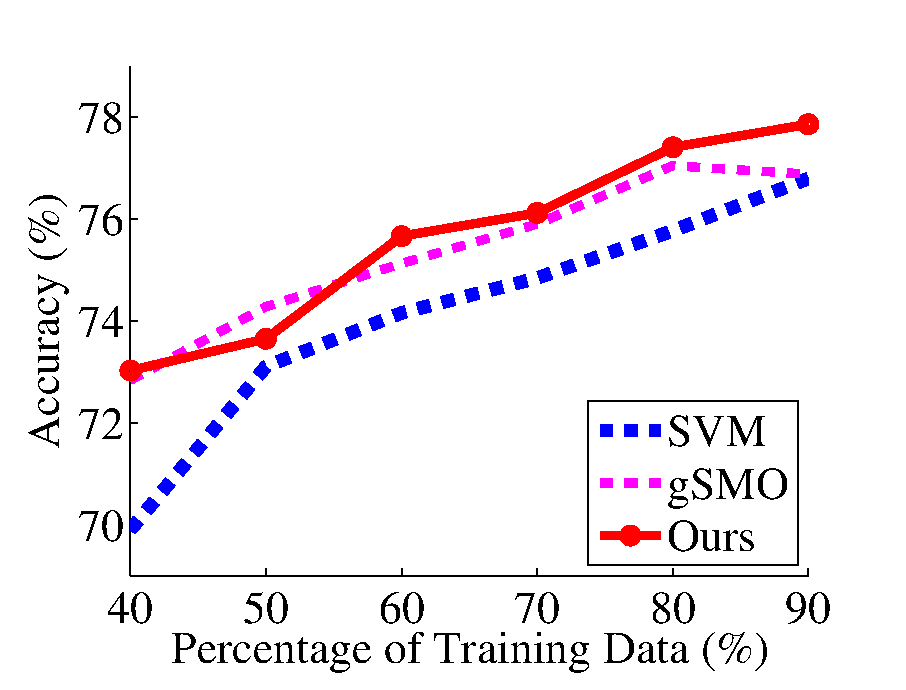
\includegraphics[width=0.46\textwidth]{./svmplus/scene15_perf.eps}
}
\subfigure[]{%{0.3\textwidth}
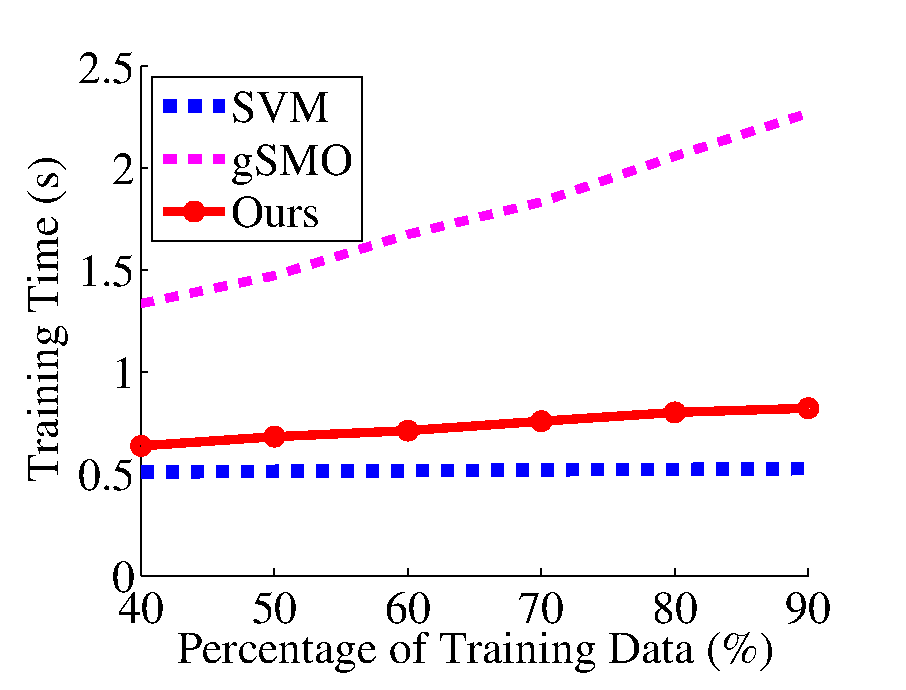
\includegraphics[width=0.46\textwidth]{./svmplus/scene15_time.eps}
}
\caption{The accuracies (Figure (a)) and the training time (Figure (b)) of different methods for solving linear SVM+ when using different number of training samples on the Scene-15 dataset.}
\label{svm:fig:linear}
\end{figure}

\noindent\textbf{Convergence:} As mentioned in
Section~\ref{sec:linear_svmplus}, our algorithm can be treated as a
special form of the linear SVM discussed in \citep{DCD_linearsvm}. So
it shares the similar convergence property as the dual coordinate
descent algorithm for linear SVM. To verify the convergence of our
algorithm, in Figure~\ref{svm:fig:mnist_obj}, we take the MNIST+ dataset
as an example to plot the objective values of our algorithm when the
number of iterations\footnote{Similarly as in LIBLINEAR, one iteration
  refers to that we pass all training samples once.} increases. It can
be observed that our algorithm converges well. The objective value
decreases very fast within the first ten iterations, and continues to
decrease as the number of iterations increases.
\begin{SCfigure}
\centering
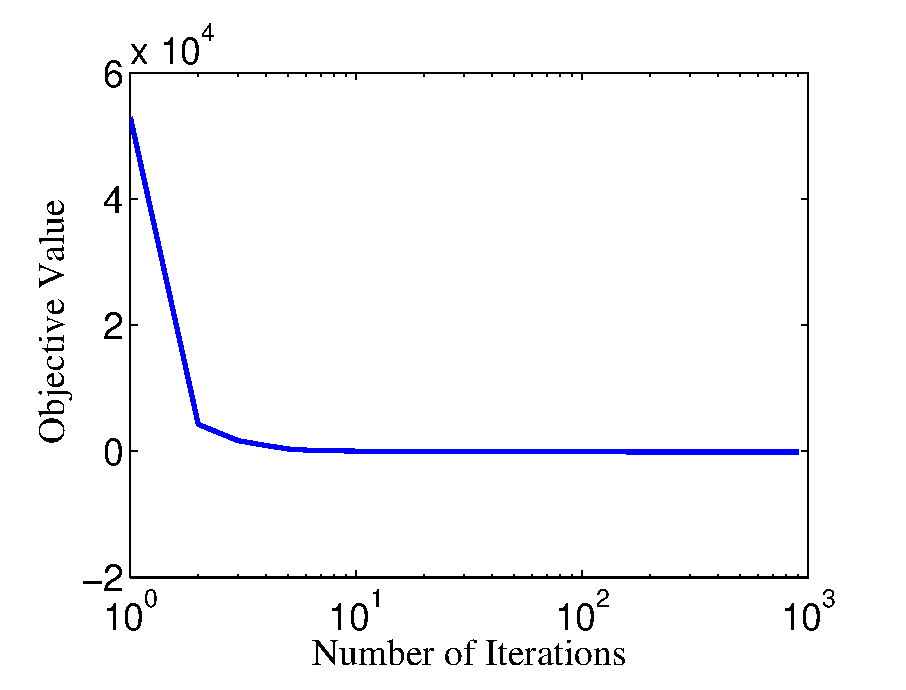
\includegraphics[width=0.56\textwidth]{./svmplus/obj_mnist.eps}
\caption{The objective of our coordinate descent algorithm for linear SVM+ on MNIST+ dataset.}
\label{svm:fig:mnist_obj}
\end{SCfigure}


\subsubsection{Experiments on Kernel SVM+}
\textbf{Experimental results:} We report the classification accuracies
and training time of all methods on two datasets when using the
Gaussian kernel in Table~\ref{tab:mnist_gaussian}. On the MNIST+
dataset, we observe that the SVM+ algorithms again achieve better
results than the baseline SVM algorithm, due to the utilizing of
poetic descriptions as privileged information. However, on the
Scene-15 dataset, \casmo and \cvx are worse than the standard SVM
method. Our $\ell_2$-SVM+ algorithm achieves better result than the
baseline algorithms, showing our new formulation for kernel SVM+ is
effective for the scene classification problem on this dataset.

In terms of the training time, we observer that our newly proposed
algorithm is the most efficient one among all SVM+ algorithms, and
generally achieves order-of-magnitude speedup over the second fastest
algorithm (\matlab on the MNIST+ dataset, and \casmo on the Scene-15
dataset). The results demonstrate the efficiency of our new
reformulation of kernel SVM+. With the reformulation, we convert it as
a one-class SVM problem, and take advantage of the existing
state-of-the-art SMO implementation in LIBSVM to solve it.

\noindent\textbf{Results using different number of training samples:}
Similarly as for the linear case, in Figure~\ref{svm:fig:nonlinear}, we
take the Scene-15 dataset to plot the classification accuracies and
training time of different methods by using different percentages of
training data. The \cvx method is not included when reporting the
training time for better visualization. We observe that our
$\ell_2$-SVM+ algorithm outperforms other SVM+ algorithms in terms of
both classification accuracy and efficiency when varying the number of
training samples.

\begin{table}[t]
\caption{ Accuracies (\%) and training time of all methods on the MNIST+ and Scene-15 dataset using the Gaussian kernel. Our results are highlighted in boldface.}
%\setlength{\tabcolsep}{3pt}
\label{tab:mnist_gaussian}
\centering
\begin{tabular}{|c|l||c|c||c|c|}
\hline
\multicolumn{2}{|c||}{}& \multicolumn{2}{|c||}{MNIST+} & \multicolumn{2}{|c|}{Scene-15}\\
\cline{3-6}
\multicolumn{2}{|c||}{}& Acc. & Time (ms) & Acc. & Time (s)\\
\hline
\multicolumn{2}{|c||}{SVM} & 92.34& 0.7& 78.79& 0.80\\
\hline
\multirow{4}{*}{SVM+}& \casmo & 92.77 & 78.8 & 77.78& 9.23\\
& \cvx & 93.14& 767.7 & 78.32& 47.16\\
& \matlab & 93.14& 54.9& 79.38& 12.07\\
& Ours & \textbf{93.15}& \textbf{1.3}& \textbf{80.57}& \textbf{1.08}\\
\hline
\end{tabular}
\end{table}

\begin{figure}
\centering
\subfigure[]{%{0.3\textwidth}
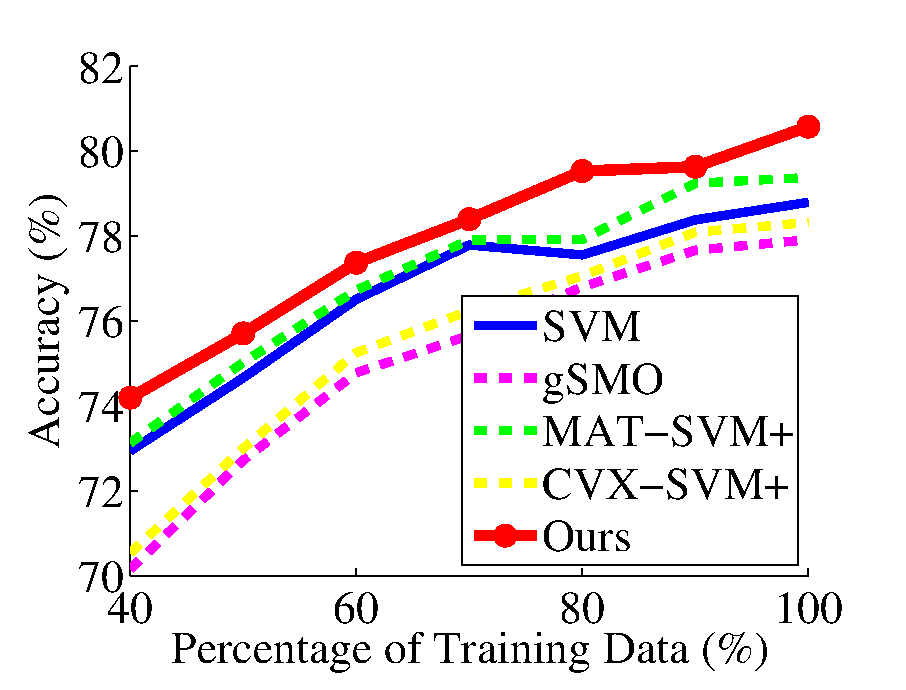
\includegraphics[width=0.46\textwidth]{./svmplus/scene15_kernel_perf.eps}
}
\subfigure[]{%{0.3\textwidth}
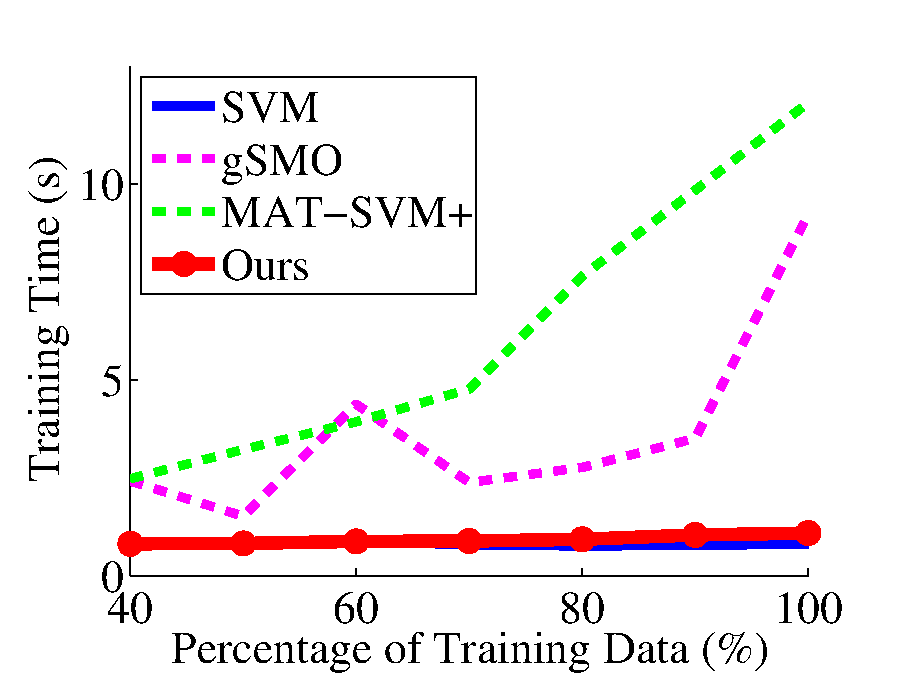
\includegraphics[width=0.46\textwidth]{./svmplus/scene15_kernel_time.eps}
}
\caption{The accuracies (Figure (a)) and training time (Figure (b)) of different methods for solving kernel SVM+ when using different number of training samples on the Scene-15 dataset.}
\label{svm:fig:nonlinear}
\end{figure}

\subsection{Web Image Retrieval}\label{sec:exp_nuswide}
In this subsection, we demonstrate the advantage of our $\ell_2$-SVM+
algorithm for solving the multiple instance learning using privileged
information problem. We employ the mi-SVM-PI algorithm proposed in
\citep{NiuIJCV2015} to evaluate different SVM+ solvers. The mi-SVM-PI
algorithm needs to iteratively solves the SVM+ problem, and
simultaneously infer the labels for training samples under MIL
constraints. We compare the mi-SVM-PI method based on our
$\ell_2$-SVM+ algorithm, with their original implementation based on
MATALB.

\noindent\textbf{Experimental setting:} It has been shown that the
textual descriptions associated with the web images are effective for
learning better classifiers using multiple instance learning
approaches~\citep{Li2014ECCV,NiuIJCV2015}.  Following \citep{Li2014ECCV,
  NiuIJCV2015}, we employ the NUS-WIDE web image dataset, which
contains $269, 648$ web images crawled from the image sharing website
\emph{Flickr}. It is officially split into a training set of 60\%
images, and test set of 40\% images. All the images are accompanied
with textual tags provided by \emph{Flickr} users. The test images are
annotated for 81 concepts. Similarly as in \citep{Li2014ECCV}, we
extract the DeCAF$_6$ features~\citep{decaf}, which leads to a
$4096$-dim feature vector for each web image. For the training data,
we also extract a $200$-dim term frequency feature from the associated
textual tags of each image, and use it as the privileged
information. $25$ positive bags (\resp, negative bags) are constructed
with each bag containing $15$ relevant images (\resp, irrelevant
images) as the training data for each concept. The Gaussian kernel is
used for the visual features, and linear kernel is used for the
textual features. The image retrieval performance is evaluated on the
test set, in which only the visual features are extracted. The average
precision based on the top-ranked $100$ test images is used for
performance evaluation, and the mean average precision (MAP) over 81
concepts is reported. Moreover, the training time of all methods over
$81$ concepts is reported for efficiency evaluation.

\noindent\textbf{Experimental results:} We report the MAPs and training time of different methods in Table~\ref{tab:nuswide}. From the table, we observe that the SVM+ methods using both solvers achieve better results than the standard SVM method, because of using additional textual information in the training process. Moreover, by incorporating the multi-instance learning approach, the MAPs of mi-SVM-PI method based on both solvers are further improved. In both cases, the methods based on our $\ell_2$-SVM+ achieve slight better results than the ones based on \matlab.

In terms of the efficiency, we observe that our $\ell_2$-SVM+ again achieves order-of-magnitude speed-up when compared with \matlab. When incorporating the multi-instance learning approach, the mi-SVM-PI based on our $\ell_2$-SVM+ uses only a bit more time than $\ell_2$-SVM+, because we only need to calculate the matrix inverse once for each concept, and iteratively solve the one-class SVM problem. In contrast, the mi-SVM-PI based on \matlab needs to iteratively solve the QP problem introduced by the SVM+ problem. Therefore, our method is more than 30 times faster than \matlab on the NUS-WIDE dataset.

\begin{table}[t]
\caption{ MAP (\%) and training time (s) of different methods on the NUS-WIDE dataset. Our results are highlighted in boldface.}
\label{tab:nuswide}
\centering
\begin{tabular}{|c|l||c|c|}
\hline
\multicolumn{2}{|c||}{}& MAP & Time (s)\\
\hline
\multicolumn{2}{|c||}{SVM} & 54.41& 9.80\\
\hline
\multirow{2}{*}{SVM+} & MAT-SVM+ & 55.63 & 204.10\\
& Ours & \textbf{55.68} & \textbf{19.44} \\
\hline
\multirow{2}{*}{mi-SVM-PI} & MAT-SVM+ & 59.11 & 765.47\\
& Ours & \textbf{59.60}& \textbf{24.26} \\
\hline
\end{tabular}
%\vspace{-5pt}
\end{table}

\section{Conclusion}
In this work, we have proposed two new algorithms for solving the
linear and kernel SVM+. By reformulating the original SVM+ method, we
obtain the dual problem with simpler constraints. Then we develop an
efficient dual coordinate descent algorithm to solve the linear SVM+
problem. We also show that the kernel SVM+ using the $\ell_2$-loss can
be converted to the one-class SVM problem, and thus can be efficiently
solved by using the SMO algorithm implemented in the existing SVM
solvers such as LIBSVM.  Comprehensive experiments on three tasks have
demonstrated the efficiency of our proposed algorithms for linear and
kernel SVM+.

%\section*{Acknowledgement}
%The work is supported by the ERC Advanced Grant Varcity ($\#273940$).
%
%{\small
%\bibliographystyle{ieee}
%\bibliography{egbib}
%}
%
%\end{document}
